\begin{figure}[!t]
\centering
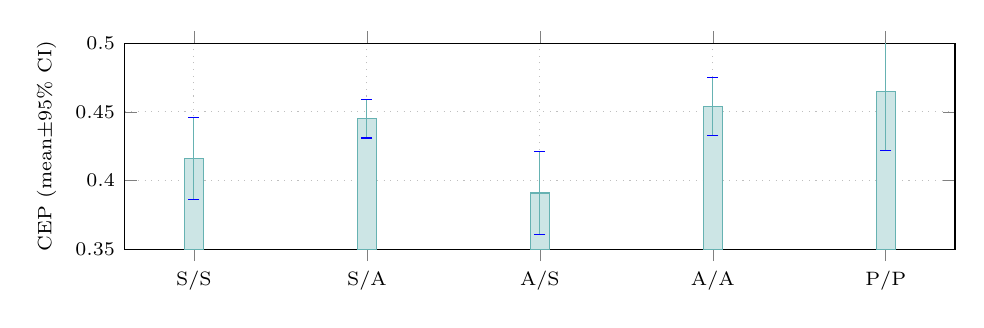
\begin{tikzpicture}
\begin{axis}[
  ybar,
  bar width=7pt,
  width=\columnwidth,
  height=4.2cm,
  ymin=0.35, ymax=0.50,
  ylabel={CEP (mean$\pm$95\% CI)},
  symbolic x coords={S/S, S/A, A/S, A/A, P/P},
  xtick=data,
  xticklabel style={font=\scriptsize},
  yticklabel style={font=\scriptsize},
  label style={font=\scriptsize},
  grid=major,
  major grid style={dotted,gray!50},
  error bars/.cd,
  ymajorgrids,
]
\addplot+[fill=teal!20, draw=teal!60, error bars/.cd, y dir=both, y explicit]
coordinates {
(S/S, 0.416) +- (0, 0.030)
(S/A, 0.445) +- (0, 0.014)
(A/S, 0.391) +- (0, 0.030)
(A/A, 0.454) +- (0, 0.021)
(P/P, 0.465) +- (0, 0.043)
};
\end{axis}
\end{tikzpicture}
\caption{Co-evolutionary pressure (CEP) on the heuristic ladder (six
seeds, $40$ episodes). CEP rises when both sides adapt (A/A, P/P),
consistent with sustained strategy change rather than a single noisy
outcome.}
\label{fig:cep-ladder}
\end{figure}
